\documentclass{article}
\usepackage[minionint,mathlf,textlf]{MinionPro} % To gussy up a bit
\usepackage[margin=1in]{geometry}
\usepackage{graphicx} % For .eps inclusion
%\usepackage{indentfirst} % Controls indentation
\usepackage[compact]{titlesec} % For regulating spacing before section titles
\usepackage{adjustbox} % For vertically-aligned side-by-side minipages
\usepackage{array, mathrsfs, mathrsfs, mhchem, amsmath} % For centering of tabulars with text-wrapping columns
\usepackage{hyperref, chemfig}
\usepackage{subfigure}
\newcommand{\Lapl}{\mathscr{L}}

\pagenumbering{gobble} 
\setlength\parindent{0 cm}
\begin{document}
\large

\section*{Introduction to fruit fly A-P patterning}

During the 1980s, in what was surely then and probably remains the most epic of genetic screens, Christiane N\"{u}sslein-Volhard and Eric Wieschaus uncovered dozens of genes involved in the anterior-posterior patterning of the fruit fly embryo. This work required studying the phenotypes of embryonic-lethal mutants and squinting at 1 mm long difformed embryos to discern anatomical features. For their efforts, both received the Nobel prize.\\

Patterning of the fruit fly anterior-posterior axis begins during oogenesis, when certain mRNAs and proteins are localized at different positions within the rather large egg. mRNAs and proteins localized in this way are called \textit{maternal effect genes}: the two most important for A-P axis specification are \textit{bicoid} mRNA at the anterior pole and \textit{nanos} mRNA at the posterior pole. After fertilization, the embryo's nuclei divide within this oocyte without forming separate cells. During this period, stored localized mRNAs begin to be transcribed, and the resulting proteins diffuse, forming concentration gradients. Bicoid and Nanos protein function by binding to target mRNAs to influence their expression: for example, translation of the anterior gene \textit{hunchback} is repressed by Nanos and transcription of \textit{hunchback} is activated by Bicoid.

\begin{center}
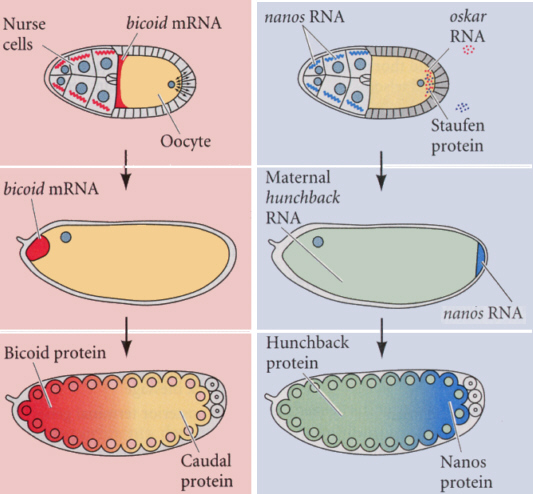
\includegraphics[width=0.5\textwidth]{gilbertmateffect.jpg}
\end{center}

About two hours after fertilization, when the embryo has thousands of nuclei, these migrate to the embryo's surface and cellularize. The concentration of the first A-P patterning factors (the maternal effect genes and their direct targets) is then ``locked in." These concentrations determine which \textit{gap genes} will be transcribed within each cell, creating regions with sharp boundaries from the continuous gradients of maternal and zygotic genes. (Note that new transcription is not a dominant factor in patterning until after cellularization.) As an example, \textit{kr\"{u}ppel} is both activated (at low concentrations) and repressed (at high concentrations) by Hunchback, and therefore is expressed in a band at roughly the middle of the embryo.

\begin{center}
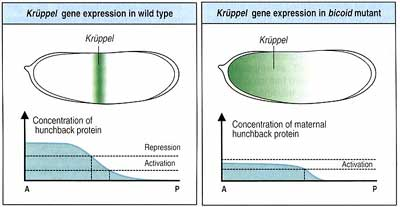
\includegraphics[width=0.5\textwidth]{kruppel.jpg}
\end{center}

The combination of gap genes in a cell then determines which \textit{pair rule genes} will be expressed. Pair rule genes are expressed in stripes in alternating (para)segments (see \textit{even-skipped} in brown and \textit{fushi tarazu} in gray, below), which would seem to imply a stripe pattern generation mechanism, but the reality is much more messy: each stripe expressing the gene may be due to a complex regulatory logic involving multiple gap genes. This logic is typically orchestrated by independent \textit{cis}-regulatory elements which then activate the gene's promoter appropriately. In a few lectures we will discuss how stripes can be generated without this sort of brute force approach, when we introduce Turing patterns.

\begin{center}
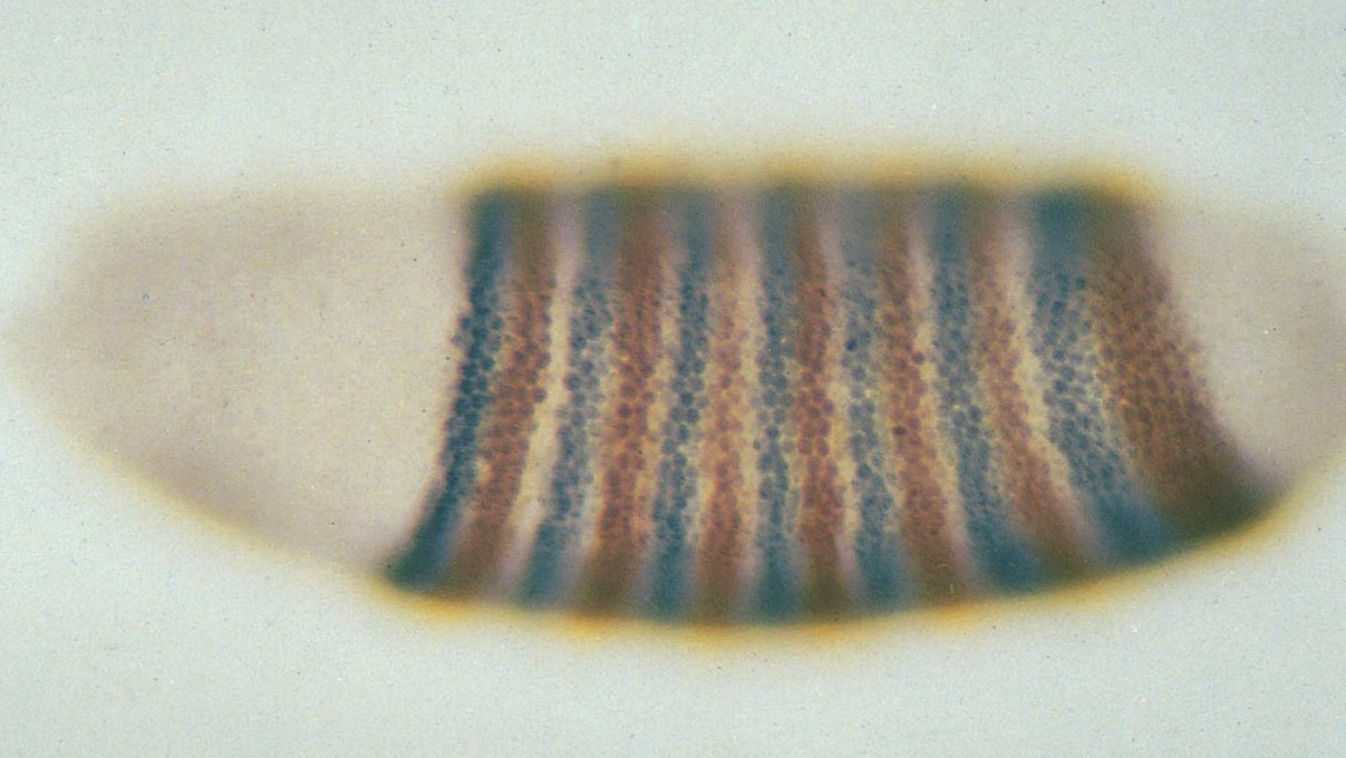
\includegraphics[width=0.5\textwidth]{evefushi.jpg}
\end{center}

The take-home message is that a continuous gradient present in the early embryo can be refined into multiple, sharp boundaries. Earlier in the course we discussed a few means by which this sort of ultrasensitive response to a protein's concentration could be achieved: an additional theme present in fruit fly A-P patterning is mutual inhibition by antagonistic and opposing gradients (here, of Bicoid and Nanos protein)\footnote{This approach is also used in dorsoventral patterning of the neural tube by sonic hedgehog vs. BMP/Wnt: the advantages it offers will be described later in the lecture.}. Though many organisms do not share the fruit fly's syncytial early development, which is required for transcription and translation factors to diffuse, gradients are nonetheless instrumental in patterning. The gradients in these cases are often of an extracellular signaling molecule diffusing from a source to a target cell. As with intracellular diffusion, the concentration of the signaling molecule at a certain location will depend on the distance from the source: the strength of the signal can thus be used to specify cell identity.\\

This type of diffusing signaling molecule is called a \textit{morphogen}. Some authors place an exacting definition on what constitutes a morphogen in order to distinguish it from signaling molecules more generally: for example, they might require that a morphogen have multiple signaling thresholds (i.e. that a cell respond differently if morphogen concentration is low vs. intermediate vs. high) as Lewis Wolpert's French Flag Model suggests. Some require that a morphogen diffuse extracellularly (many definitions state that morphogens ``act upon cells"), whereas many others consider Bicoid to be the first protein convincingly demonstrated to act as a morphogen\footnote{Driever and N\"{u}sslein-Volhard reported this in 1988, almost seven decades after Thomas Hunt Morgan proposed the existence of a morphogen and more than three decades after Alan Turing coined the term. As of this writing, no wikipedia page exists for Bicoid despite its historical and biological importance.}. At any rate, you'll find that the general principles described here for Bicoid are applicable regardless of the chosen definition of morphogen.

\section*{Diffusion with degradation from a constant source}

In the early fruit fly embryo, \textit{bicoid} mRNA is localized to the anterior pole where its translation begins at fertilization. Bicoid protein is then free to diffuse through the syncytium toward the posterior pole of the embryo. Bicoid protein is relatively unstable, so that when formulating a reaction-diffusion equation for its concentration gradient, it is important to account for its degradation. This gives a Helmholtz PDE:
\[ \frac{\partial c}{\partial t} = D \frac{\partial^2 c}{\partial x^2} - \gamma c \]
After some time Bicoid diffusion and degradation are expected to balance such that the concentration gradient becomes constant. The general solution for equations of this form can be found by multiplying through by $dc/dx$ and proceeding as follows:
\begin{eqnarray*}
\int \left[ \frac{\partial c}{\partial x} \cdot \frac{\partial^2 c}{\partial x^2} - \frac{\gamma c}{D} \frac{\partial c}{\partial x} \right]\, dx & = & \int \, dx \\
\frac{\left( \frac{\partial c}{\partial x} \right)^2}{2} - \frac{\gamma c^2}{2D}   & = & k_1\\
 \frac{\partial c}{\partial x} & = & \pm \sqrt{2k_1 + \frac{\gamma}{D} c^2}\\
 \int \frac{dc}{\sqrt{2k_1 + \frac{\gamma}{D} c^2}} & = & \pm \int \, dx\\
 \arccos \left( c \sqrt{\frac{1}{2k_1}} \right) & = & \pm ix\sqrt{\frac{\gamma}{D}} + k_2 \\
 c & = & A \cos \left( \pm i x \sqrt{\frac{\gamma}{D}} + \phi \right)
\end{eqnarray*}
Using the angle addition and exponential identities for cosine, we can rewrite the general solution as:
\[ c(x) = c_1 e^{-x/ \lambda} + c_2 e^{x/\lambda} \]
where $\lambda = \sqrt{D/\gamma}$ is the length scale of the system. At steady-state, $c(0)$ is some non-negative constant and $c(\infty) \to 0$. These boundary conditions imply that at steady state:
\[  c(x) = c(0) e^{-x\sqrt{\gamma/D}} \]
Variation in the number of mRNAs will affect c(0) linearly: fortunately the variation in the number of mRNAs between embryos is approximately 10\% (Petkova et al., 2014), only as variable, it transpires, as the protein gradient. (Houchmandzadeh et al. (2005) note, however, that ``if the human nose were positioned by such a
morphogen, we would find it in some individuals on the
torso and in some on top of the head.") \\

An interesting problem is that this exponential profile falls off rather rapidly, yet Bicoid is used for A-P patterning in fruit fly embryos that span an order of magnitude in egg length. Imagine that you were to take a fruit fly egg, make it three times as larger, then try to manipulate some other parameter of this system so that the Bicoid gradient scaled, i.e., Bicoid protein reached $x$\% of its maximal level at the same fractional length in the larger egg as in the original, for all $x$. It would not be ideal to simply increase $c(0)$ because you could only correct one value of $x$ at a time by this approach: in other words, you could never make both the head and the thorax proportionally the right size at the same time in this way. However, it is at least easy to imagine how you would tune $c(0)$. Alternatively, you could manipulate the exponential rate constant. You probably cannot find a way to increase the diffusion coefficient of Bicoid artificially (but see below concerning Bicoid dwell time in nuclei). Instead, you could decrease $\gamma$ -- that is, stabilize the Bicoid protein -- if you can figure out how. This does not appear to have been the approach taken by evolution in the larger embryos of some \textit{Drosophila} sister clades (Gregor et al., 2008). \\

Evolution suggests time and again that we should not rely on our intuition of how ``hard" or ``easy" it is to evolve something: our collective engineering aptitude is usually not flattered by the result. Instead, the Ma lab at Cincinnati has taken the approach of experimentally evolving \textit{D. melanogaster} strains with large and small eggs through artificial selection, achieving roughly 33\% increase/decrease in size relative to wildtype (Cheung et al., 2011 and Miles et al., 2011). The evolved strains have features scaled proportionately to their length. By examining Bicoid gradients in these embryos (Cheung et al., 2014), they have demonstrated that these strains primarily achieved proper scaling through modification of the exponential rate rather than $c(0)$. This modification may not be the result of a heritable mutation: it could instead represent an inherent scaling property of the system.

\section*{Bicoid retardation by nuclear entry}

It is not clear, in the experimental evolution example above, whether the exponential rate constant was changed through genetic modification or was simply the consequence of an existing method to scale $\lambda$ appropriately for an egg's shape. Since the Bicoid gradient is not the only feature of the fruit fly that needs to scale as the egg length changes, the latter seems more plausible. Indeed, there are potential fitness benefits to evolving a system that automatically scales, since there is variation in embryo size at deposition, and we presume canalization of proportions is important for viability.\\

One potential explanation that has been explored experimentally is that diffusion of transcription factors may be retarded by their entry into nuclei. Like most transcription factors, Bicoid contains a nuclear localization sequence that allows it to enter nuclei which it encounters; Bicoid is released when the nucleus dissolves during mitosis. In the \textit{Drosophila} sister clades \textit{Calliphora} and \textit{Lucilia}, embryos are roughly three times larger and wider than those of \textit{D. melanogaster}, but the number of nuclei at the time of cellularization is the same:  if the number of nuclei is limiting for Bicoid diffusion, the effective value of $D$ will be higher in the larger embryos because of the greater distance between nuclei (Gregor et al., 2008). An increase in $D$ was observed when embryos expressed an mRNA encoding GFP-NLS at the anterior pole of larger vs. smaller embryos: unfortunately, this was not able to fully account for scaling.

\section*{Scaling of cytoplasmic convection}

An alternative hypothesis is that convection of cytoplasm helps carry Bicoid protein away from the anterior pole. Cytoplasmic streaming has been directly observed in \textit{Drosophila} embryos and simulation results suggest it may contribute to extending the profile of Bicoid along the embryo's periphery (Hecht et al., 2009). Simulation results show that if the magnitude of the flow scales proportionally with the embryo's length, this approximately scales the Bicoid gradient as desired.


\section*{Non-linear degradation}

Another source of variation likely to be encountered in real embryos is variation in $c(0)$ due to differences in mRNA expression levels. (For Bicoid, the variation is on the order of 10\% of the mean, but this is expected to differ for other transcripts and organisms.) Changes in $c(0)$ shift the exponential concentration profile left or right, as can best be visualized on log-log axes [draw at board].\\

One way to make scaling robust to this type of variation is to posit that the diffusing protein be degaded non-linearly. This occurs, for example, if the protein forms dimers and only the dimers are degraded. Then our reaction-diffusion equation becomes:
\[ \frac{\partial c}{\partial t} = D \frac{\partial^2 c}{\partial x^2} - \gamma c^2 \]
with the same boundary conditions as before:
\begin{eqnarray*}
 \frac{\partial^2 c}{\partial x^2} & = & \frac{\gamma}{D} c^2\\
\int  \frac{\partial^2 c}{\partial x^2} \cdot \frac{\partial c}{\partial x} \, dx & = & \int  \frac{\gamma}{D} c^2 \cdot \frac{\partial c}{\partial x} \, dx\\
\left(\frac{\partial c}{\partial x} \right)^2 & = &  \frac{2 \gamma}{3D} c^3 + k_1\\
\int \frac{dx}{\sqrt{\frac{2 \gamma}{3D} c^3 + k_1}} & = & \pm \int \, dx
\end{eqnarray*}
Solutions for $y$ are given by the Weierstrass elliptic functions which suggests an ansatz solution (see Eldar et al., 2003) of the form $c(x)= k_1/(x+k_2)^2$. We can verify quickly that this solution satisfies our reaction-diffusion equation:
\[ D \frac{\partial^2 c}{\partial x^2} - \gamma c^2 = \frac{6D k_1}{\left(x+k_2\right)^4} - \frac{\gamma k_1^2}{\left(x+k_2\right)^4} = 0 \]
if we choose $k_1=6D/\gamma$ and, to meet the boundary condition at the source, $k_2=\sqrt{6D/\gamma c(0)}$. This power law solution falls off less steeply than the exponential profile associated with a linear degradation term. Moreover, for $x \gg k_2$, this concentration profile approaches $c\approx k_1/x^2$ regardless of $c(0)$, so this profile is robust to variation in mRNA concentration at points sufficiently far from the source.

\section*{Opposing morphogen gradients}

A philosophically simple mechanism for scaling is provided by a system in which two morphogens are secreted from opposite poles, and cell fate is defined by the ratio between the two signals. In the case where the morphogens do not interact (Houchmandzedah et al., 2005), as long as degradation is non-linear and of identical order for the two morphogens, the ratio between morphogens is robust to variation in production rate and the majority of the embryo's length will exhibit robust scaling with embryo size. Requiring that the degradation term's order be exactly identical, however, is an example of parameter fine-tuning. A further challenge -- how to read out the ratio between the two morphogens accurately -- remains even if the parameters are perfectly tuned (Ben-Zvi et al., 2010). An opposing approach is that instead of having two non-interacting morphogens diffusing from either end, a morphogen diffuses from one pole and its inhibitor from the other (McHale et al., 2006).

\section*{Morphogen shuttling}

The \textit{Drosophila} dorsoventral axis is patterned in a conceptually-related way as you learned earlier in the semester while preparing for your second paper discussion. As a recap, you saw that an initial gradient in the nuclear localization of Dorsal causes a subset of cells to ingress and form mesoderm, with the cells left in the ventral ectoderm eventually becoming neural and epidermal cells. Midline secrete Spitz, signaling to the nearest neighbors to degrade Yan and assume a neural fate. The border of the neural and epidermal regions was made more distinct by zero-order ultrasensitivity in the degradation of Yan.\\

Now we take a look at the opposite side of the embryo, where a different morphogen (a BMP called Decapentaplegic\footnote{The name derives from the fifteen imaginal discs in which major organs and appendages of the adult develop in the pupa.} or Dpp) is secreted. Instead of being secreted only by a row of cells directly along the midline as is the case for Spitz, Dpp is secreted approximately uniformly in a broad region. Diffusion and degradation of Dpp in this scenario would create a fairly uniform concentration profile along the embryo's dorsal midline, which would not help these cells to distinguish their identity.\\

An extracellular mechanism called morphogen shuttling is used to ``tighten up" the morphogen gradient. A second protein called short gastrulation (Sog), secreted in the region adjacent to the dorsal region, binds to Decapentaplegic and inhibits its binding to receptors. Binding to Sog is also thought to paradoxically increase the effective diffusion coefficient of Dpp by preventing it from dawdling at its own receptors. The Sog-Dpp complex is a target for a third protein called Tolloid (Tll) which is uniformly expressed: Tll binds the complex and proteolytically cleaves Sog, releasing Dpp. Because Sog helps Dpp travel farther then releases it again, Sog is considered to act as a shuttle.\\

Although the Sog-Dpp complex diffuses freely, on average it will tend to carry Dpp toward the embryo's dorsal midline. This is because Dpp is more likely to initially bind Sog laterally where Sog concentration is high, and if by chance it moves farther away from the midline, more likely to rebind another Sog molecule after being released from the first one.  At the midline, where Sog concentration is low, Dpp will thus accumulate to higher levels than would be expected with a uniform field of morphogen production alone. (See Shilo et al., 2013 for a review.)\\

It turns out that this mechanism results not just in a sharper gradient, but in robustness to several variables (see Eldar et al., 2002). Representing [Sog] by $s$, [Sog-Dpp] by $c$, and $[Dpp]$ by $d$, and assuming that the concentration of tolloid ($t$) is constant, the equations defining this reaction-diffusion system are:
\begin{eqnarray}
\frac{\partial s}{\partial t} & = & D_{s} \nabla^2 s - k_b s d \label{eqn1}\\
\frac{\partial c}{\partial t} & = & D_{c} \nabla^2 c + k_b s d - \lambda t c \label{eqn2}\\
\frac{\partial d}{\partial t} & = & - k_b s d + \lambda t c \label{eqn3}
\end{eqnarray}
Notice that we have assumed free Decapentaplegic does not diffuse at all. A steady-state solution is found by setting all of these equations equal to zero. Plugging \ref{eqn3} into \ref{eqn2}, we find the general solution for $c(x)$:
\[ D_{c} \nabla^2 c \implies c(x) = a_1 + a_2 x \]
But if we define $x=0$ to be the midline of the embryo, then $c$ must be an even function by symmetry, so $c(x)$ is jspatially constant. From equation \ref{eqn3}, we have that $d = \lambda t c / k_b s$. Plugging this into equation \ref{eqn1}, we get that:
\[ D_{s} \nabla^2 s = D_{s} \nabla^2 \left( \frac{\lambda t c}{k_b d} \right) =  \lambda t c \implies \nabla^2 \left( \frac{1}{d} \right) = \frac{k_b}{D_s} \]
with the division by $\lambda t c$ allowable since all of these quantities are constant. Then we can solve for d by simple integration to obtain:
\[ d(x) = \frac{1}{\frac{k_b}{D_s} x^2 + b_1 x + b_2} = \frac{1}{\frac{k_b}{D_s} x^2 + b_2} \]
where symmetry again determines that $b_1=0$. Sufficiently far from the midline, we have
\[ d(x) \approx \frac{D_s}{k_b x^2} \]
with all the same advantages as the power law distribution we saw previously for non-linear degradation of Bicoid.

\section*{Expansion-repression feedback}

A general mechanism for generating scaling which relates conceptually to shuttling is the expansion-repression mechanism. An expander $e$ is imagined to aid the diffusion of a morphogen $m$; high morphogen levels repress the expression of the expander. Binding to the expander also helps the morphogen to avoid degradation, as would be plausible if the expander prevented receptor binding and thus receptor-mediated endocytosis (Ben-Zvi et al., 2010).\\

If we assume that the morphogen's concentration profile initially follows a power law, than the expander will be expressed at higher levels at the opposite poll and fall off near the origin, where morphogen concentration is highest [drawn at board]. Morphogens at the tail of the distribution will thus be aided in their diffusion. Eventually a new power law distribution is reached where expander production is inhibited everywhere (the rapidly-diffusing expander's concentration profile will then become uniform). Expansion-repression feedback appears to be at play during dorsoventral patterning in the frog.\\

Expansion-repression feedback works through a form of integral control. The accumulated expander concentration represents the total ``error" (extent of the region where expander is still being expressed) over time.



\end{document}